\documentclass{standalone}
\usepackage{tikz}
\usepackage{graphicx}
\usetikzlibrary{shapes}

\newdimen\imageheight % goes into the preamble

\settoheight{\imageheight}{%
  \includegraphics[width=\textwidth,keepaspectratio]{example-image}%
}

\begin{document}
  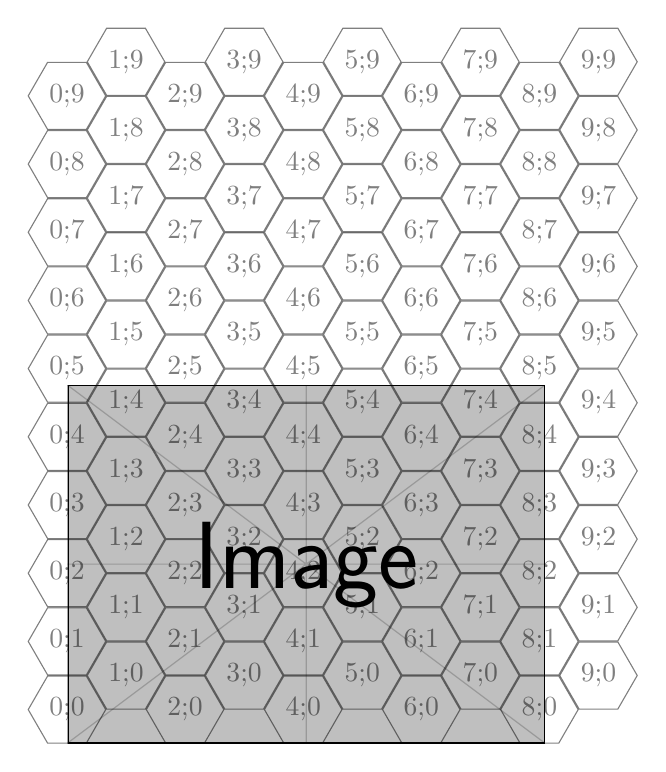
\begin{tikzpicture} [hexa/.style= {shape=regular polygon,
                                     regular polygon sides=6,
                                     minimum size=28pt, draw,
                                     inner sep=0,anchor=south,
                                     opacity=.5}]

\node[anchor=south west,inner sep=0] (image) at (0,0) {\includegraphics[width=0.5\textwidth]{example-image}};
      \foreach \j in {0,...,9}{% 
           \ifodd\j 
               \foreach \i in {0,...,9}{\node[hexa] (h\j;\i) at ({\j/2+\j/4},{(\i+1/2)*sin(60)}) {\j;\i};}        
          \else
               \foreach \i in {0,...,9}{\node[hexa] (h\j;\i) at ({\j/2+\j/4},{\i*sin(60)}) {\j;\i};}
          \fi}
  \end{tikzpicture}

\end{document}      
